
\clearpage
\section{Die Adressliste benutzen}
\label{bkm:Ref443738751}
In der Adressliste werden auf einfache Art und Weise sämtliche im CUBE PA erfassten Personen und Organisationen/Firmen angezeigt. Mittels der Filterfunktion können Einträge rasch gefunden werden.

\vspace{\baselineskip}

Für die Benutzung der Adressliste sind folgende Eigenschaften zu berücksichtigen:

% \liststyleWWviiiNumxiii
\begin{itemize}
\item
Ist ein Benutzer des CUBE PA entsprechend berechtigt, kann er in der Adressliste neue Personen und neue Organisationen erfassen oder bestehende Einträge bearbeiten.

\item
Personen, welche auf diese Weise erfasst wurden, stehen automatisch in allen Personen-Auswahlfeldern zur Verfügung (z.B. Pendenzen). Jedoch können sich diese neu erfassten Personen im CUBE PA nicht anmelden. Wird dies erwünscht, kann der Administrator behilflich sein, resp. ist mit dem CUBE PA Support Kontakt aufzunehmen (siehe Kapitel
\ref{bkm:Ref443502661}).

\item
Wird einer Person einer Organisation zugewiesen, erscheint in der Adressliste automatisch die Organisationsadresse. Ist dies z.B. wegen abweichenden Organisationsstandorten nicht erwünscht, kann im Bearbeitungsfenster der Person eine spezifische Adresse hinterlegt werden.

\item
Bei Personen, welche sich aktiv in CUBE PA einloggen können, kann die Organisationszugehörigkeit aus Sicherheitsgründen (Zugriffsrechte) nur durch den Administrator geändert werden. Melden Sie solche Mutationen bitte dem Administrator, resp. dem CUBE PA Support (siehe Kapitel \ref{bkm:Ref443502661}).

\item
Organisationseinträge, welche in der Adressliste erfasst wurden, stehen nicht automatisch als Anbieter oder Auftraggeber im Beschaffungswesen zur Verfügung. Sollen Organisationen auch im Beschaffungswesen angezeigt werden, muss dies durch den Administrator entsprechend konfiguriert werden.

\item
Nebst den Standard-Feldern können benutzerdefinierte Felder hinzugefügt werden (Konfiguration nur durch CUBE PA Support). Diese Felder können anschliessend ebenfalls gefiltert und exportiert werden.

\end{itemize}

\textbf{Personen und Benutzer:} In der Adressverwaltung wird vorwiegend von 'Personen' gesprochen. 'Benutzer' unterscheiden sich von 'Personen' darin, dass sie sich in CUBE PA anmelden können. Jede 'Person' kann entsprechend zu einem 'Benutzer' konfiguriert werden. Diese Anpassungen werden im Modul 'Benutzerverwaltung' vorgenommen. Dazu braucht es jedoch administrative Rechte. Wenden Sie sich bei Bedarf an den CUBE Support.

\pagebreak
\subsection{Finden von Personen oder Organisationen in der Adressliste}

\begin{wrapfigure}[7]{l}{6.5cm}   % [x] Wie manche Zeile soll sich um die Grafik "brechen"
  \vspace{-35pt}      % Grundwert war 20; mit 30 schön oben beim Text ausgerichtet
  \begin{center}
    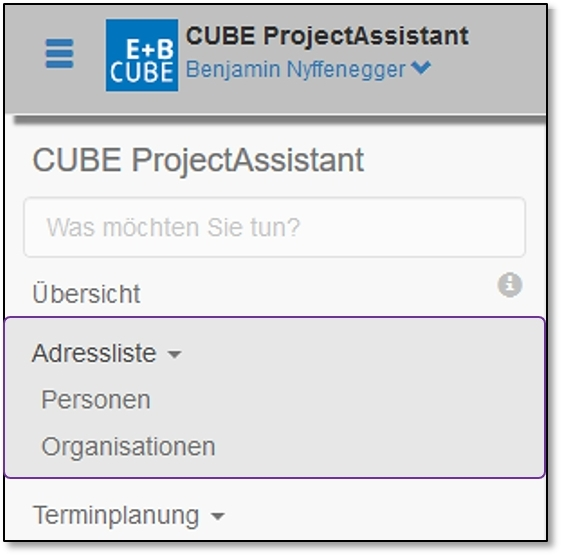
\includegraphics[width=1\linewidth]{../chapters/03_Adressliste/pictures/3-1_Menu_Adressliste.jpg}
  \end{center}
  \vspace{-20pt}
  \caption{Adresslistenmenü}
  \vspace{-10pt}
\end{wrapfigure}

Wählen Sie aus dem Menü links den Punkt 'Adressliste' aus. Als Unterpunkte sehen Sie 'Personen' und 'Organisationen'. Wählen Sie das Gewünschte aus.\\
Im Folgenden wird der Umgang mit 'Personen' erläutert. Die Bedienweise bezieht sich aber mehrheitlich auch auf 'Organisationen'.

\vspace{4cm}

Es erscheint eine Liste mit sämtlichen im CUBE PA hinterlegten Adressen von Personen oder Organisationen:

\begin{figure}[H]
\center{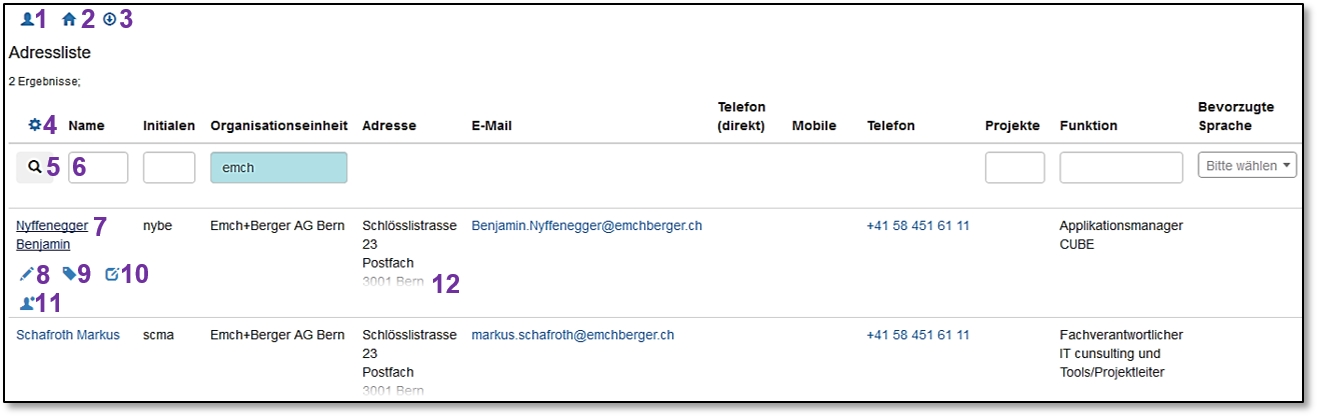
\includegraphics[width=1\linewidth]{../chapters/03_Adressliste/pictures/3-1_Adressliste_Uebersicht.jpg}}
\caption{Die Übersicht der Adressliste}
% \label{fig:speciation}
\end{figure}

Oben links haben Sie die Möglichkeit, neue Personen 
\includegraphics[height=12pt]{/Icons/Person.jpg} oder Organisationen 
\includegraphics[height=12pt]{/Icons/Haus.jpg} zu erfassen. Beachten Sie die Eigenschaften, welche eingangs des Kapitels aufgeführt wurden (Kapitel \ref{bkm:Ref443738751}). \newline
Mit Klick auf 
\includegraphics[height=12pt]{/Icons/ListeGenerieren.jpg} \col{(3)} werden die gefilterten Daten als Exceldatei exportiert. So können Sie die Daten beispielsweise für einen Serienbrief verwenden oder Massenänderungen vornehmen und anschlissend die Tabelle wieder importieren. 

\vspace{\baselineskip}

\textbf{Hinweis:} Die Exportfunktion wird nur bei den Personen unterstützt.

\textbf{Hinweis:} Für die Importfunktion beachten Sie die Hinweise im Kapitel \ref{bkm:Ref2018090701}.

\vspace{\baselineskip}

Mit dem Konfigurations-Symbol 
\includegraphics[height=12pt]{/Icons/SpaltenEinst.jpg} \col{(4)} können Spalten ein- und ausgeblendet werden, um die Tabelle übersichtlicher zu gestalten. \\
Für die Suche / Filterung verwenden Sie die bestehenden Suchfelder \col{(6)} der Spalten (Wenn Sie benutzerdefinierte Felder verwenden, können Sie auch bei diesen Feldern suchen / filtern.). Sobald Sie Eingaben machen, wird die Datenbank durchsucht und das Suchresultat angepasst.

\vspace{\baselineskip}

\textbf{Hinweis:} Mit einem Doppelklick auf das Lupen-Symbol 
\includegraphics[height=12pt]{/Icons/Lupe_kl.jpg} \col{(5)} werden die Suchbegriffe gelöscht und der Filter zurückgesetzt.

\vspace{\baselineskip}

Mit einem Klick auf den Namen \col{(7)} oder die Organisation werden weitere Optionen eingeblendet. Mit dem vCard-Symbol 
\includegraphics[height=12pt]{/Icons/vCard.jpg} \col{(8)} wird vom ausgewählten Datensatz eine vCard für Outlook geöffnet oder gespeichert. Fürs Bearbeiten eines Datensatzes klicken Sie auf das Bearbeiten-Symbol 
\includegraphics[height=12pt]{/Icons/bearbeiten.jpg} \col{(9)}. Abhängig von den Berechtigungen erscheint ein weiteres Symbol 
\includegraphics[height=12pt]{/Icons/User.jpg} \col{(10)}. Mit Klick darauf werden die Usereinstellungen geöffnet (Anpassungen bei Berechtigungen, Zugehörigkeiten etc.) - diese Option ist ausschliesslich für Superuser und Administratoren.

\vspace{\baselineskip}

Standardmässig werden für eine bessere Übersicht nur die ersten Zeilen eines Datensatzes angezeigt \col{(11)}. Sie können jedoch auf den 'ausgegrauten' Text klicken, um sämtliche Angaben anzeigen zu lassen.

\clearpage
\subsection{Neue Personen oder Organisationen in der Adressliste erfassen}
\label{bkm:Ref2018071901}
Berechtigte Benutzer können in der Adressliste neue Personen oder Organisationen erfassen oder bestehende Einträge ändern:

\vspace{\baselineskip}

\begin{tabular}{cc} %{cl}
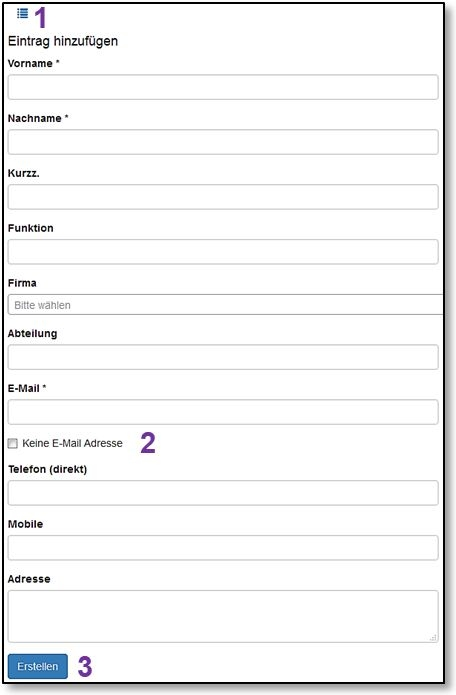
\includegraphics[width=0.49\textwidth]{../chapters/03_Adressliste/pictures/3-2_Personeneintraege.jpg} & 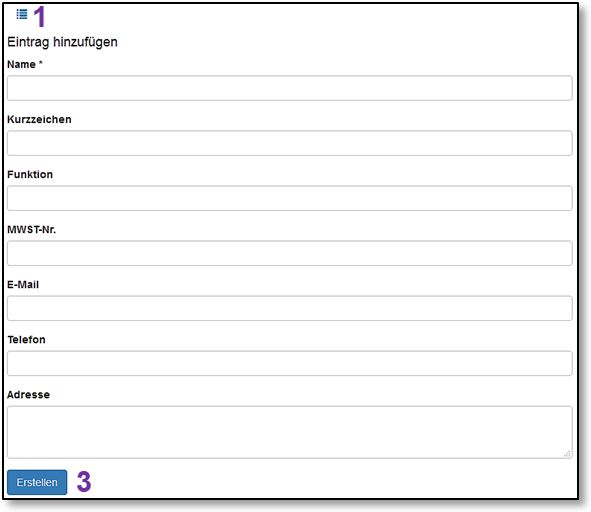
\includegraphics[width=0.49\textwidth]{../chapters/03_Adressliste/pictures/3-2_Firmeneintraege.jpg} \\
Personeneinträge & Organisationseinträge \\
\end{tabular}

% \begin{figure} 
%      \subfigure{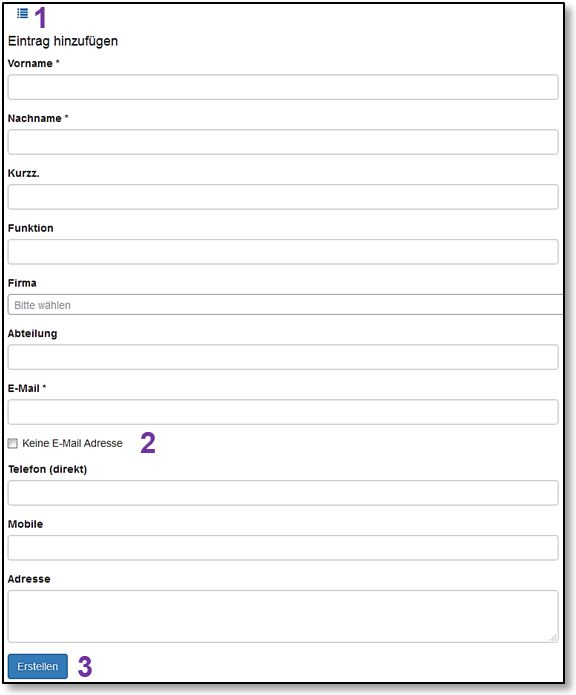
\includegraphics[width=0.49\textwidth]{32_Personeneintraege.jpg}} 
%      \subfigure{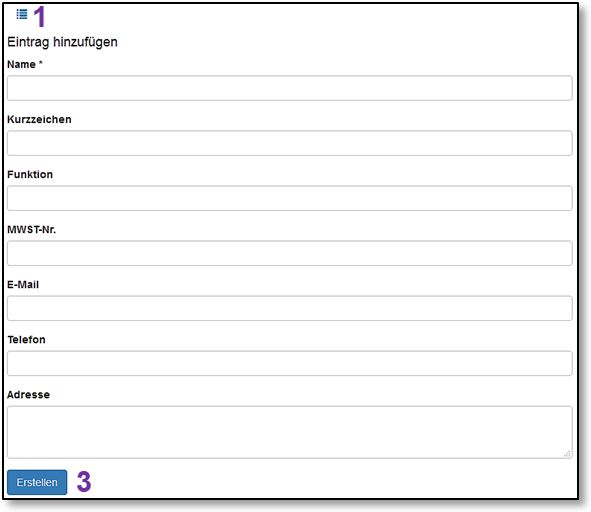
\includegraphics[width=0.49\textwidth]{32_Firmeneintraege.jpg}} 
% \caption{Die verschiedenen Eingabemasken der Adressliste} 
% \end{figure}

\vspace{\baselineskip}
Alle Felder mit * sind Pflichtfelder und müssen ausgefüllt werden. Kann / soll keine E-Mail-Adresse hinterlegt werden, kann dieses Pflichtfeld mittels einem Häkchen 'Keine E-Mail-Adresse' \col{(2)} umgangen und leergelassen werden. Nach dem Eingeben der gewünschten / bekannten Feldern wird der Datensatz mit 'Erstellen' \col{(3)} gespeichert und steht anschliessend in der Adressliste zur Verfügung. Wurde bei einem bestehenden Eintrag auf das Bearbeitungssymbol 
\includegraphics[height=12pt]{/Icons/Bearbeiten.jpg} geklickt, wird die gleiche Maske (siehe oben) geöffnet. Alle bereits hinterlegten Daten sind in den entsprechenden Feldern vorhanden und können geändert werden. Wie oben eingangs des Kapitels bereits vermerkt, kann bei einer Person die Organisations-/ Firmenzugehörigkeit aus Sicherheitsgründen (Zugriffsrechte) nicht, resp. nur durch den Administrator geändert werden.

\vspace{\baselineskip}

Durch Klick auf das Listensymbol 
\includegraphics[height=12pt]{/Icons/Listensymbol_zurueck.jpg} \col{(1)} gelangen Sie zurück zur Adressliste.

\vspace{\baselineskip}

\textbf{Hinweis zu Zusatzfeldern:} Es ist möglich sogenannte 'custom fields' (benutzerdefinierte Felder) in der Adressliste zu hinterlegen und die bestehenden Datenbankfelder dadurch zu erweitern. Für weitere Auskünfte oder das Bereitstellen solcher Datenbankfelder kontaktieren Sie bitte den CUBE-Support.

\subsection{Personen- und Organisationseinträge mutieren}

Wählen Sie im Menü links unter Adressliste die gewünschte Liste aus (Personen oder Organisationen). Die Übersicht erscheint:

\begin{figure}[H]
\center{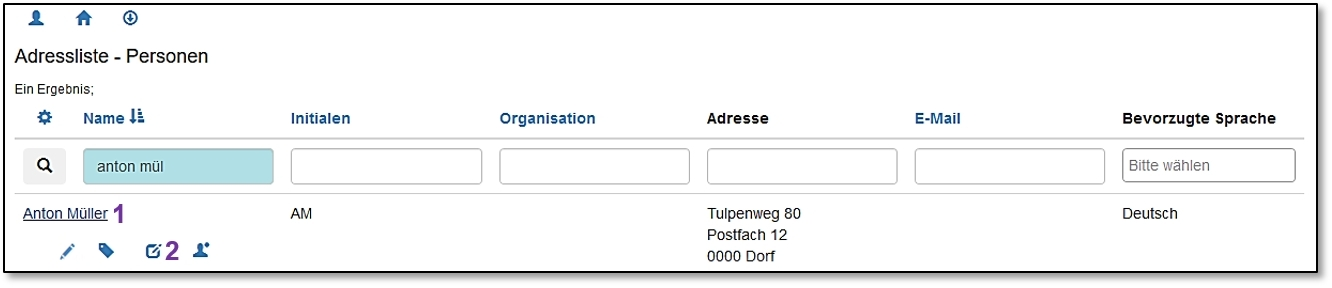
\includegraphics[width=1\linewidth]{../chapters/03_Adressliste/pictures/adr_AdresseBearbeiten.jpg}}
\caption{Eintrag bearbeiten}
% \label{fig:speciation}
\end{figure}

Suchen Sie den zu mutierenden Eintrag und klicken Sie auf den Namen oder die Organisation \col{(1)}. Die Optionen werden geöffnet. Mit Klick auf das Bearbeiten-Symbol 
\includegraphics[height=12pt]{/Icons/Bearbeiten.jpg} \col{(2)} wird die Eingabemaske des entsprechenden Eintrages geöffnet:

\begin{figure}[H]
\center{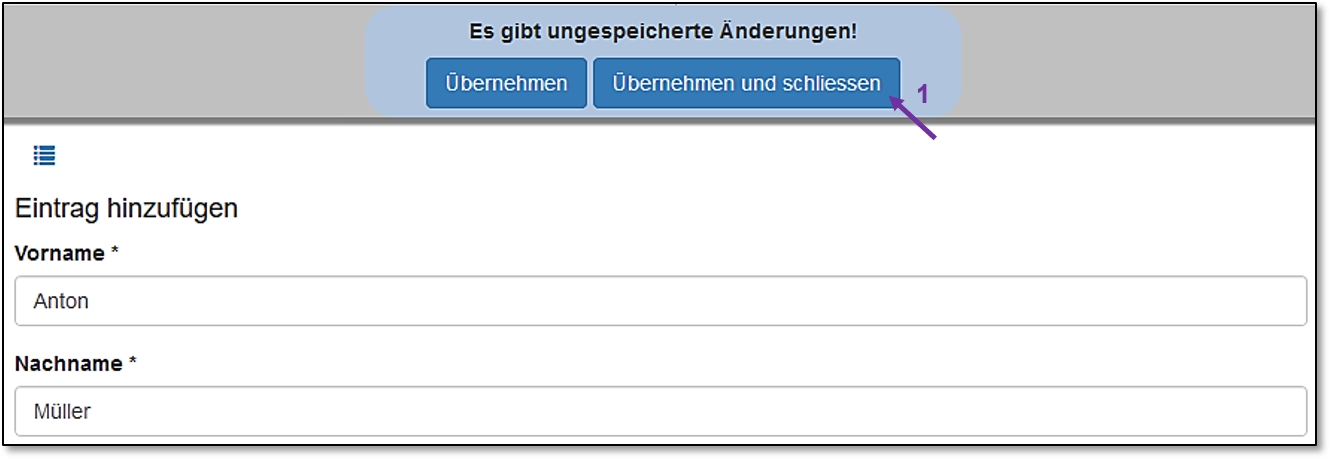
\includegraphics[width=1\linewidth]{../chapters/03_Adressliste/pictures/adr_AdressenBearbeiten_u_schl.jpg}}
\caption{Eintrag speichern und schliessen}
% \label{fig:speciation}
\end{figure}

Wurden die benötigten Änderungen vorgenommen, können Sie mit Klick auf 
\includegraphics[height=12pt]{/Icons/ueb_schliessen.png} \col{(2)} die Änderungen speichern und die Maske schliessen. Die Übersicht wird wieder angezeigt. Falls Sie nur eine Zwischenspeicherung der Änderunge machen wollen, klicken Sie auf 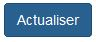
\includegraphics[height=12pt]{/Icons/B_Uebernehmen.jpg}.

\pagebreak
\subsection{Personen- und Organisationseinträge mit der Inline-Funktion ändern}

Öffnen Sie wie gewohnt die Adressliste für Personen oder Organisationen.

\begin{figure}[H]
\center{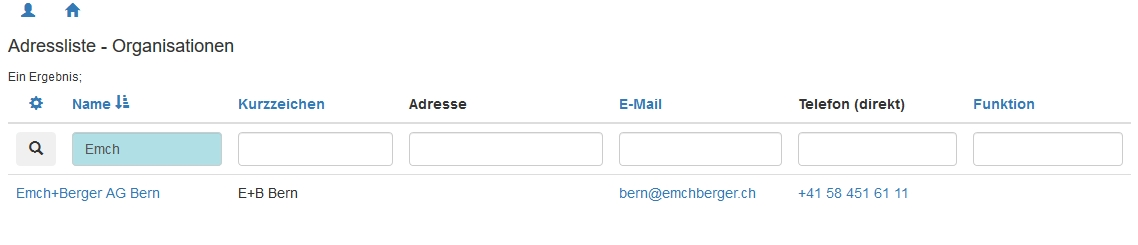
\includegraphics[width=1\linewidth]{../chapters/03_Adressliste/pictures/temp_inline1.jpg}}
\caption{Einträge in der Übersicht bearbeiten}
% \label{fig:speciation}
\end{figure}

Nun können Sie beim Datensatz, welcher bearbeitet werden soll, einen Doppelklick machen (Beachten Sie oben im Bild den umrahmten Bereich). 

\vspace{\baselineskip}

\textbf{Hinweis:} Klicken Sie für die Inline-Bearbeitung nicht auf die Emailadresse und nicht auf die Telefonnummer, da bei diesen Feldern eine Funktion hinterlegt ist, welche eine neue Email erstellt oder eine Telefonverbindung aufbaut.

\vspace{\baselineskip}

Nach dem Doppelklick werden nun die Eingabefelder sichtbar:

\begin{figure}[H]
\center{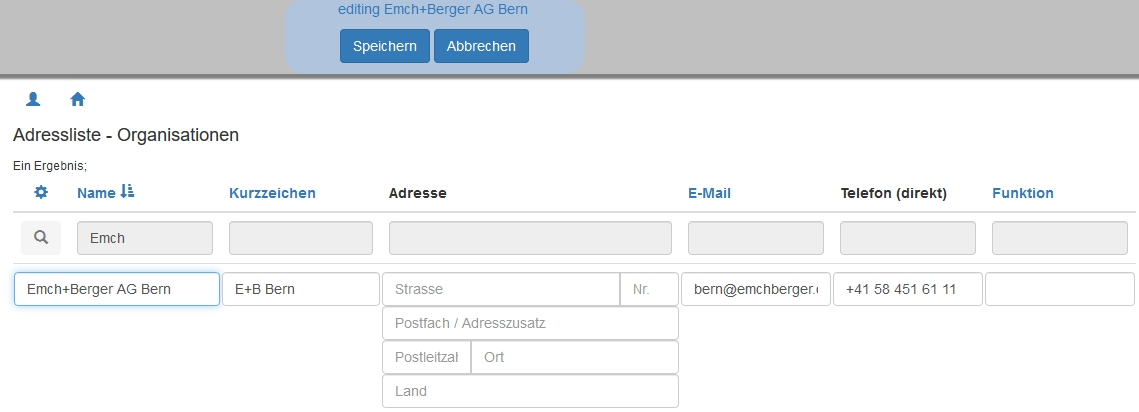
\includegraphics[width=1\linewidth]{../chapters/03_Adressliste/pictures/temp_inline2.jpg}}
\caption{Einträge in der Übersicht bearbeiten}
% \label{fig:speciation}
\end{figure}

Sie können nun die Änderungen vornehmen und mittels dem 
\includegraphics[height=14pt]{/Icons/Speichern.png}-Button oder mit erneutem Doppelklick im umrahmten Bereich die Änderungen speichern.

\vspace{\baselineskip}

\textbf{Hinweis:} Wenn Sie den Editiermodus nicht verlassen und einen weiteren Datensatz mit Doppelklick bearbeiten möchten, erscheint folgende Meldung:

\begin{figure}[H]
\center{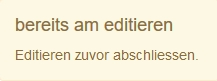
\includegraphics[width=.25\linewidth]{../chapters/03_Adressliste/pictures/temp_inline3.jpg}}
\caption{Meldung - Eintrag in Bearbeitung}
% \label{fig:speciation}
\end{figure}

Speichern Sie wie oben beschrieben den in Bearbeitung stehenden Eintrag ab, bevor Sie einen neuen Datensatz bearbeiten wollen.

\vspace{\baselineskip}

\textbf{Hinweis:} Wenn Sie mit dem 
\includegraphics[height=12pt]{/Icons/SpaltenEinst.jpg}-Symbol Spalten ausgeblendet haben, werden diese beim Bearbeiten nicht eingeblendet. Achten Sie demnach darauf, dass vorgängig alle benötigten Spalten eingeblendet sind.

\vspace{\baselineskip}

\textbf{Hinweis:} Wurde bei einem Personeneintrag eine Firmenadresse hinterlegt, wird dies entsprechend angezeigt. Sie haben jedoch die Möglichkeit eine personenbezogene Adresse zu hinterlegen. Diese wird mit Priorität angezeigt. Wird diese wieder gelöscht, erscheint wieder die hinterlegte Organisationsadresse. Die Organisationsadresse können Sie hier nicht ändern.

\vspace{\baselineskip}

\textbf{Hinweis:} Wurde keine Emailadresse hinterlegt, wird dies entsprechend angezeigt. Um der Person eine Emailadresse hinzuzufügen, wählen Sie den Weg via Klick auf das 
\includegraphics[height=12pt]{/Icons/bearbeiten.jpg}-Symbol. Die Eingabemaske wird geöffnet. Entfernen Sie das Häkchen bei 'Keine E-Mail Adresse' und tragen Sie die E-Mail Adresse ein.
